
\documentclass[a4paper, 11pt]{book}

\usepackage[utf8]{inputenc}      % Pour gérer correctement les accents
\usepackage[T1]{fontenc}
\usepackage[francais]{babel}     % Indentation et style français
\usepackage[babel=true]{csquotes}
\usepackage[bindingoffset=1cm, hmargin=2cm, vmargin=3cm, headheight=14pt]{geometry}
\usepackage{graphicx}
\usepackage{textcomp}      % Pour les symboles comme 'degré'
\usepackage{tocloft}       % Config des espacements des titres
\usepackage{amsmath}       % Pour les équations
\usepackage{numprint}      % Pour les nombres en style français
\usepackage{units}         % Pour \unit
\usepackage{gensymb}       % Pour le degré en math
\usepackage{subfig}        % Pour les sous-figures
\usepackage{hyperref}      % Pour faire des liens dans le document
\usepackage{fancyhdr}      % Pour l'en-tête et le pied de page
\usepackage{dsfont}		   % Pour une jolie lettre pour l'esnemble des réels
\usepackage{setspace}
\usepackage{listings} 
\usepackage[vlined, french, nofillcomment]{algorithm2e}            

\title{Création d'un réseau d'objets intelligents, génériques et dynamiques : SmartDevCom}
\author{Thomas \textsc{Impery} \\ Cyrille \textsc{Pierre}}

\setlength{\parskip}{10pt}             % Espace entre les paragraphes

\makeatletter  % Pour les variables @author et @date

% Configuration de l'en-tête et du pied de page
\fancypagestyle{plain}{%
   \renewcommand{\headrulewidth}{0pt}
   \renewcommand{\footrulewidth}{.4pt}
   \fancyhf{}
   \fancyfoot[C]{\thepage}
   \fancyfoot[L]{\@author}
   \fancyfoot[R]{\@date}}
   
\renewcommand{\headrulewidth}{.4pt}
\renewcommand{\footrulewidth}{.4pt}
\fancyhf{}
\fancyhead[L]{\leftmark}
\fancyfoot[C]{\thepage}
\fancyfoot[L]{\@author}
\fancyfoot[R]{\@date}
\pagestyle{fancy}

% Config page blanche
\let\origdoublepage\cleardoublepage
\newcommand{\clearemptydoublepage}{%
  \clearpage
  {\pagestyle{empty}\origdoublepage}%
}

\renewcommand{\baselinestretch}{1.2}   % interligne à 1.5
   

\begin{document}
	
\begin{titlepage}
   \noindent
   \setstretch{1.0}
   \begin{minipage}{.45\textwidth}
      
\includegraphics[width=.8\textwidth]{img/logo_isima.png}
      \\[.5cm]
      \textbf{I}nstitut \textbf{S}upérieur \\
      d'\textbf{I}nformatique, de \\
      \textbf{M}odélisation et de \\
      leurs \textbf{A}pplications
      \\[.5cm]
      \footnotesize
      Campus des Cézaux \\
      24 avenue des Landais \\
      BP 10125 \\
      63173 AUBIERE Cedex
   \end{minipage}
   \hspace{.03\textwidth}
%    \begin{minipage}{.45\textwidth}
%       \begin{flushright}
%       \end{flushright}
%    \end{minipage}
   \\[.5cm]
   %
   \begin{center}
      Rapport d'ingénieur \\
      Projet de 3\ieme{} année \\
      Filière : Informatique des systèmes embarqués
      \rule{\textwidth}{.3pt}
      \LARGE \textbf{\textsc{\@title}}
      \rule{\textwidth}{.3pt}
      \hbox{\vspace{3cm}} \\
%       \includegraphics[width=.5\textwidth]{img/os32c.png}
   \end{center}
   {\large \textbf{\@author}}
   \\[.5cm]
   Tuteur : Michel \textsc{Cheminat} \\
   Référent : Christian \textsc{Laforest} \\
   \begin{flushright}
      \footnotesize
      Soutenance : 10/03/2016 \\
      Projet de 120 heures par personne
   \end{flushright}
\end{titlepage}

   \makeatother
   
   \clearemptydoublepage
   
   \frontmatter   % Numérotation romaine minuscule
   
   \chapter*{Remerciements}

Nous remercions M. Cheminat qui a su nous guider pour fixer des objectifs concrets.
   \clearemptydoublepage
   
   
\chapter*{Résumé}
Le but de ce projet de dernière année est de réaliser une \textbf{intelligence artificielle} capable de communiquer avec nous, cela dans le but de créer un réseau d'objets intelligents sans limite physique au niveau du support de communication de l'objet, de sa position et enfin de son type. Ce réseau permettra donc de pouvoir parler avec un objet pouvant se trouver à quelques mètres de nous, mais aussi à l'autre bout de la planète. Il nous autorisera de la même manière de pouvoir allumer la lumière de notre maison, mais aussi de pouvoir observer l'évolution de la température de notre piscine. Le dernier but de ce projet est de pouvoir être indépendant de la technologie de communication.

Afin de réaliser ce projet, il faut en premier lieu savoir ce qui caractérise un \textbf{objet intelligent}. Après avoir listé les fonctionnalités que peut avoir n'importe quel type d'objet, il faut mettre en place un \textbf{protocole} afin de pouvoir communiquer avec eux. La construction de ce protocole passe en premier lieu par la \textbf{classification} de l'ensemble des objets que l'on sera à même de pouvoir créer. Ensuite, il faut porter ce protocole sur les objets intelligents. Ces objets sont constitués d'un microcontrôleur \textbf{Mbed} et d'un ou plusieurs capteur(s) et/ou actionneur(s). Le protocole doit aussi être portée sur une application \textbf{Android}. Cette application permet d'utiliser la \textbf{reconnaissance vocale} d'Android, afin de pouvoir interagir avec les objets autour de nous, de la manière la plus naturelle possible.
	
   \paragraph{Mots clés}: Intelligence artificielle, objet intelligent, protocole, classification, Mbed, Android, reconnaissance vocale.
		% ...
   
\clearemptydoublepage
   
 \chapter*{Abstract}
The aim of this last year's project, is to realize an \textbf{artificial intelligence} able of communicating with us, in order to create a network of smart objects without any physical limit about the communication support, his position and finally his type.

Looking forward to that goal, in the first place, one must know what define a \textbf{smart object}. Having listed the features that can have any type of object, one must set a \textbf{protocol} to communicate with them. In the first place, the building of this protocol is a \textbf{classification} of the whole objects we are able to create. Then, one must brings this protocol on the smart objects. These objects are made of a \textbf{Mbed} microchip, and one or several sensors and/or actuators. The protocol must be carried on an \textbf{Android} application aswell. This application allows us to use Android \textbf{voice recognition}, in order to interact with the objects around us, in the most natural way.
 
   \paragraph{Keywords:}Artificial intelligence, smart object, protocol, classification, Mbed, Android, voice recognition.

   \clearemptydoublepage
   
   \tableofcontents
   \clearemptydoublepage
   
   \listoffigures
   \clearemptydoublepage
   
   \chapter*{Introduction}

Aujourd'hui les objets connectés sont partout. Dans notre frigo, dans notre portable, et même dans notre 
brosse à dents. Tous ces systèmes sont capables de parler, mais tous avec un langage différent, impossible à 
comprendre pour les autres. Tous ces objets ne sont que des entités dispersées, sans intelligence propre, là 
où normalement nous parlons d'objets intelligents. Tous les constructeurs créent un protocole différent pour 
faire communiquer leurs propres objets, impliquant une non compabilité avec les objets d'un concurrent, ce qui 
est préjudiciable pour les gens souhaitant acquérir un panel d'objets de diverses marques. Ainsi il serait 
dans l'intérêt des utilisateurs d'avoir un moyen de redonner l'intelligence à ses objets, et de réussir à tous 
les faire communiquer entre eux, peu importe son origine.

De nos jours, Internet est le réseau le plus connu, et un des réseau des plus abouti. Nous parlons d'Internet 
des objets pour parler des objets connectés au sens large, mais ceux-ci n'utilisent pas encore de protocole 
qui permettent un acheminement des données tel que Internet peut le faire. Ainsi notre projet se basera sur 
les travaux qu'Internet a pu apporter, afin de réaliser un protocole similaire, dédié à l'Internet des 
objets. Cela dans le but de créer un réseau virtuel se basant sur un réseau physique déjà existant, grâce à 
Internet lui-même, et des technologies tel que le Bluetooth, afin de relier tous nos objets entre eux.
   \clearemptydoublepage   

   \mainmatter    % Numérotation arabe

   \chapter{Automatisation de la maison}

\section{L’intelligence des objets}
	\subsection{Définition d’un objet connecté}
Aujourd'hui les objets connectés font partis de notre quotidien, et peuvent réaliser énormément 
d'actions différentes. Globalement on peut dire qu'un objet connecté, ou l'internet des objets, représente 
l'extension d'Internet à l'ensemble des objets de notre monde physique. Cela permet de donner de 
l'intelligence à des objets, afin qu'ils puissent nous communiquer différentes informations 
(\textbf{Capteurs}), ou bien exécuter différentes choses (\textbf{Actionneurs}). Ces événements peuvent être 
réalisés manuellement ou automatiquement selon le besoin.

Malgré tout, ces objets ne sont sémantiquement pas connectés entre eux pour plein de raisons différentes. 
SmartDevCom permet de réaliser un ensemble d'objet tous connectés entre eux. Un objet connecté est constitué 
d'un ou plusieurs capteur(s) ou actionneur(s).
% 		Définition générale + notre version par rapport au projet
	\subsection{Les capteurs}
	
Les capteurs sont tous les objets qui permettent d'obtenir une information sur l'environnement. Ces capteurs 
permettent par exemple de connaître la température de la pièce, de savoir si la lumière est allumée, ou si la 
porte d'entrée est ouverte.

Ces capteurs permettent une interaction simpliste avec l'environnement puisqu'ils permettent seulement 
d'obtenir une information physique. Ainsi, l'utilisation d'un capteur est très simple, puisqu'il suffit de 
lui demander d'envoyer la valeur qu'il contient.
% 		les types de capteurs
% 		leurs caractéristiques au sein d’un objet connecté
	\subsection{Les actionneurs}
	
Les actionneurs sont tous les objets qui permettent de réaliser une action. Ces actionneurs permettent par 
exemple d'ouvrir les volets, d'allumer la climatisation, ou bien d'allumer la lumière.

Ils permettent une interaction plus prononcée avec l'environnement, comparativement aux capteurs, étant donné 
qu'ils ont besoin de paramètres pour réaliser l'action voulue. Par exemple si l'on souhaite allumer une 
lumière intelligente, il faudra préciser l'intensité lumineuse, ainsi que la couleur de celle-ci.
% 		les types de capteurs
% 		leurs caractéristiques au sein d’un objet connecté

\section{La communication des objets}
	\subsection{Présentation des technologies de communication}
Actuellement, il existe de nombreux protocoles réseaux qui permettent la communication entre les différents 
objets. Ces protocoles établissent des normes, afin de pouvoir dialoguer entre différents acteurs.

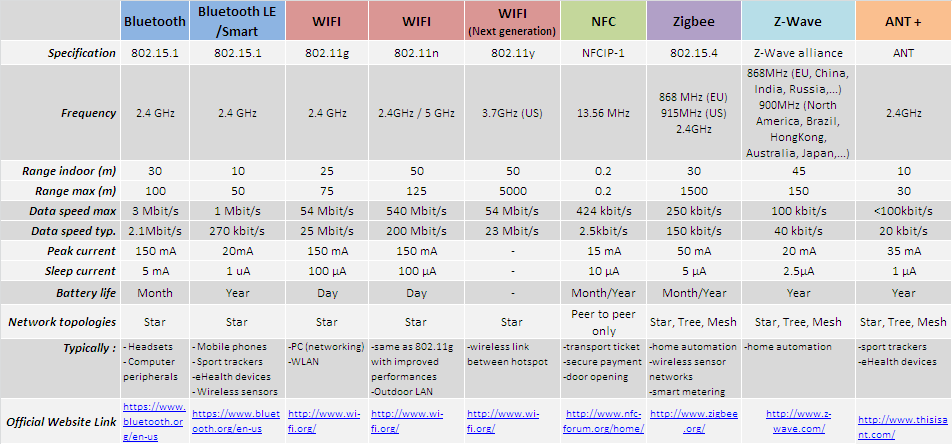
\includegraphics{img/tableau-total.png} 

Tous ces protocoles ont leur avantages et leur inconvénients. Malgré tous ces protocoles, on peut voir qu'il 
existe principalement deux familles :

\paragraph{Les protocoles très énergivores}qui permettent de faire transiter des données avec un débit très 
élevé. Cette cadence est permise grâce à une fréquence trés élevé. Cette fréquence a par conséquent 
l'inconvénient de très peu passer les obstacles, et donc d'émettre sur une courte distance.

\paragraph{Les protocoles peu énergivores}qui possèdent des caractéristiques opposées. En effet ils 
permettent de faire transiter des données avec un faible débit, sur une grande distance grâce à une fréquence 
bien moindre.

C'est donc la deuxième famille qui est la plus utilisée pour l'internet des objets, puisqu'ils n'ont pas 
besoin d'envoyer beaucoup de données, ont besoin d'envoyer le plus loin possible, et surtout d'avoir le plus 
d'autonomie possible. Les protocoles les plus réprésentatifs de cette famille, sont le Bluetooth Low Energy 
(ou BLE), le Zigbee, et Z-Wave. Ces deux derniers sont relativement onéreux et compliqués à mettre en place, 
c'est pourquoi le BLE est le protocole le plus démocratisé de cette famille.

% 		wifi, bluetooth, BLE, zig-bee, …
% 		quelques caractéristiques (débit, portée, consommation)
	\subsection{Les différentes topologies de réseaux}
En plus des différents protocoles, il existe aussi des topologies différentes pour créer un réseau d'objets.

	    \subsubsection{Etoile}

\includegraphics{img/StarNetwork.svg.png}

	    \subsubsection{P2P}
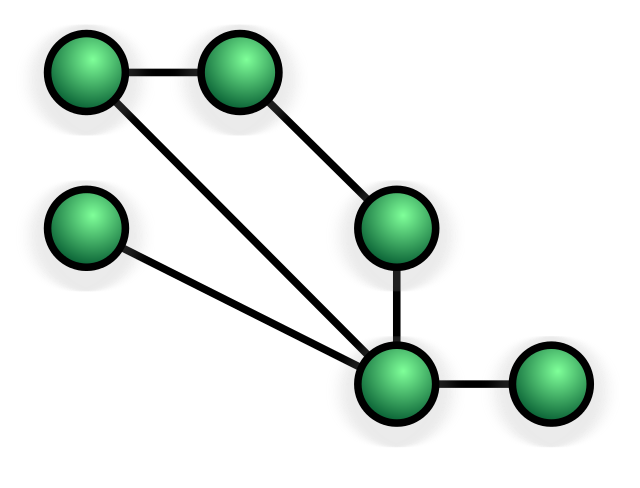
\includegraphics{img/NetworkTopology-Mesh.svg.png}

	    \subsubsection{Arbre}
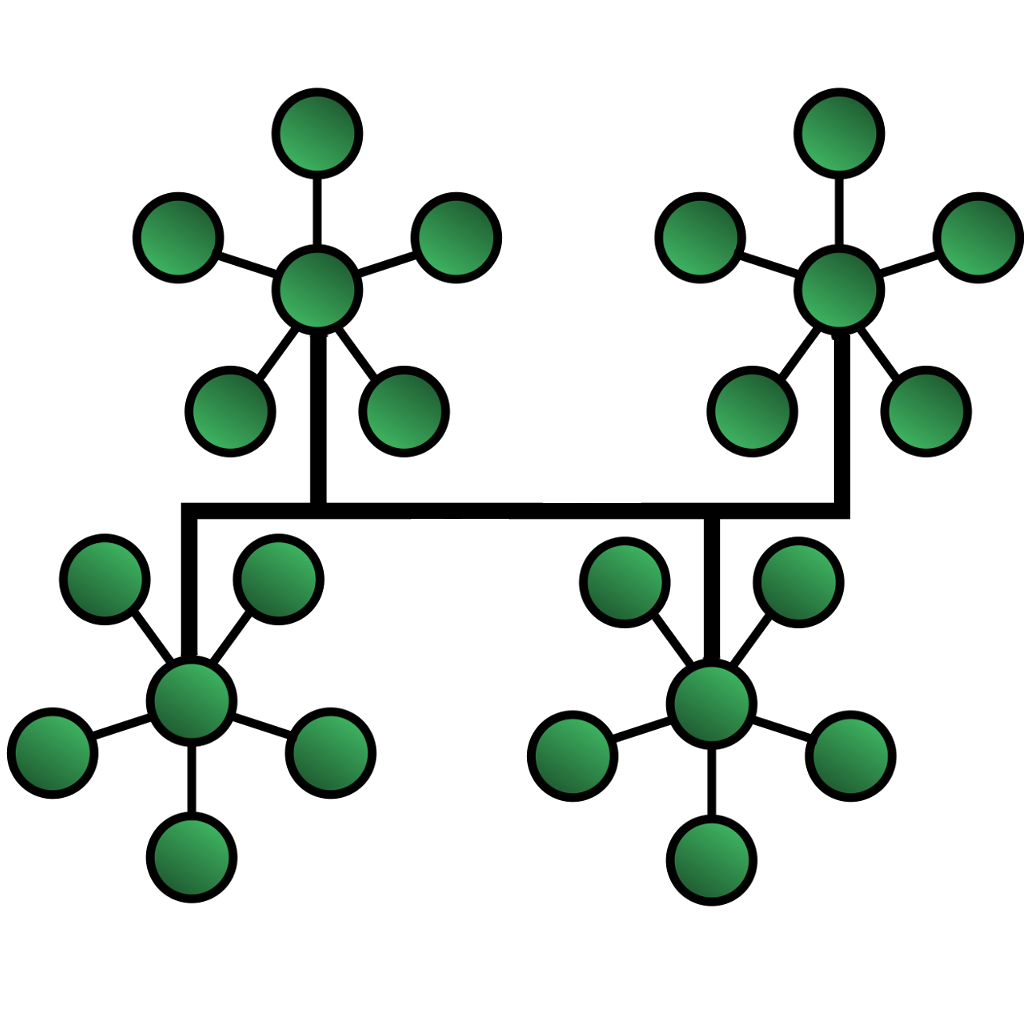
\includegraphics{img/TreeTopology.png}


% 		p2p, étoile, mesh, ...
% 		lien avec les technos
	\subsection{Application du réseau à la domotique}
% 		les technologies les plus adaptées à la domotique
% 		exemples d’architecture réseau dans une maison (avec ou sans mélange de technos)

\section{La centralisation de l’intelligence : Jarvis}
	\subsection{Vision macroscopique d’un système domotique}
% 		les conséquences de la connexion des objets
	\subsection{Les scénarios}
% 		explication sur l’intérêt de la connexion des objets
% 		exemples d’utilisations
	\subsection{Analyse et anticipation de requêtes}
% 		analyse plus poussée des données : statistiques, interprétations des mesures
% 		intégration d’intelligence artificielle
% 		exécution de tâches de façon autonomes
% 		les limites

   \clearemptydoublepage
   
   \chapter{Mise en place du protocole de communication}
	Le premier chapitre de se rapport a présenté les principales idées que l'on souhaite mettre en 
	place pour avoir une architecture d'objets dynamique et générique. On va maintenant s'intéresser
	à la manière dont on peut les réaliser.


\section{Les protocoles existants}
	Il existe une multitude
	% A ECRIRE, A ECRIRE	, A ECRIRE, A ECRIRE, A ECRIRE, A ECRIRE

	\subsection{Zigbee}
	% A ECRIRE, A ECRIRE	, A ECRIRE, A ECRIRE, A ECRIRE, A ECRIRE
	\subsection{Z-Wave}
	% A ECRIRE, A ECRIRE	, A ECRIRE, A ECRIRE, A ECRIRE, A ECRIRE
	\subsection{Alljoyn}
	% A ECRIRE, A ECRIRE	, A ECRIRE, A ECRIRE, A ECRIRE, A ECRIRE
	
	% IMPORTANT : explication de pourquoi on a pas pris un protocole existant :
	%  - ne correspond pas forcément à toute les fonctionnalités que l'on souhaite mettre en place
	%  - est difficilement adaptable avec les outils que l'on a (mbed, attiny, bluetooth Bolutek)

\section{Le réseau virtuelle}
	Nous allons maintenant nous intéresser aux caractéristiques du protocole qui a été
	développé dans ce projet. L'un des points clés de la mise en place d'objets pour la domotique 
	est la communication avec ceux-ci. Ces objets doivent en effet être "connectés" pour que l'on
	puisse les contrôler ou recevoir des messages de leur part. Il est donc nécessaire de mettre en 
	place une architecture réseau qui puisse lier ces objets de façon efficace. Mais la mise en place
	de ce réseau n'est pas forcément évidente. Si l'on souhaite être indépendant du support de 
	communication, il faut mettre en place des moyens de lier des objets de supports différents. Il 
	est également possible de communiquer avec des objets mobiles. Cela signifie que l'architecture 
	du réseau doit également être dynamique. C'est pourquoi il est indispensable d'avoir un protocole
	capable de gérer tous ces détails.
	
	\subsection{Architecture du réseau}
% 		définition d’un réseau (uniquement 1 support de communication)
% 		description de la connexion des réseaux
% 		exemples d’architecture de réseau virtuel
		Pour bien comprendre comment est structuré un réseau d'objets, il faut d'abord s'intéresser 
		à une architecture simple ne faisant qu'intervenir un seul support de communication. La figure
		\ref{netStar} représente un réseau créé par des objets connectés possédant une interface Wifi.
		En utilisant du Wifi \emph{Point d'Accès}, un des objets fait office de serveur (\emph{C}) 
		sur lequel les autres objets clients viendront se connecter. Avec cette architecture de 
		réseau, l'ensemble des objets peuvent parler entre eux mais tous les messages passent par 
		\emph{C}. Cette connexion est complètement transparente à l'utilisation puisqu'elle 
		directement gérée par le protocole IP. La communication consistera simplement à créer une
		\emph{socket} TCP ou UDP entre deux objets. Ils pouront alors parler sans avoir à s'occuper
		du transport de leurs messages.
		
		\begin{figure}[!ht]
         \centering
         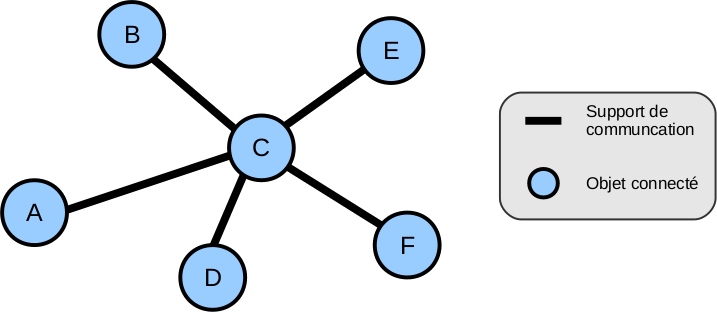
\includegraphics[width=.8\textwidth]{img/reseau_etoile.png}
         \caption{Exemple d'architecture réseau d'un point d'accès Wifi (topologie en étoile).}
         \label{netStar}
      \end{figure}

      Si l'on prend cette fois-ci l'exemple d'une architecture formée par d'objets utilisant 
      ZigBee (figure \ref{netGraph}), on remarque que les objets ne sont pas lié à un unique objet
      mais à l'ensemble des objets qui sont à sa portée. Un objet peut donc communiquer directement
      avec un objet voisin mais également avec des objets plus distants s'il existe un chemin dans
      le graphe du réseau. Encore une fois, toute cette architecture est déjà gérée nativement par
      les composants ZigBee. Cependant son utilisation est un peu différente d'une utilisation 
		d'objets en Wifi. Certains protocoles de communication utilisant du ZigBee (par exemple Xbee) 
		ne permettent pas d'envoyer des messages à une cible précise. C'est la totalité des objets qui
		sont présent dans le réseau ZigBee qui recevront le message. Cela signifie qu'il faudra gérer
		la cible dans le message en lui-même. Cette méthode peut être un inconvénient puisqu'il
		complexifie la création des messages mais il offre un avantage au niveau du transport de ces
		messages.
      
      \begin{figure}[!ht]
         \centering
         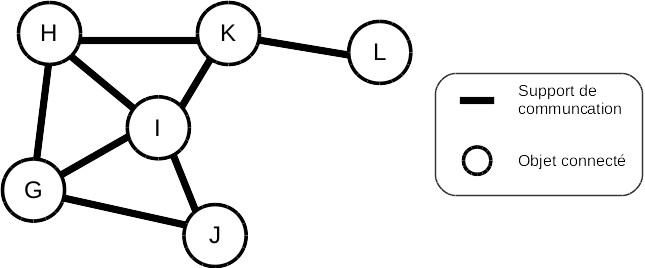
\includegraphics[width=.8\textwidth]{img/reseau_graphe.png}
         \caption{Exemple d'architecture réseau d'objet en ZigBee (topologie en maillage).}
         \label{netGraph}
      \end{figure}
      
      Ces deux architectures sont les plus courantes dans les technologies de communication sans
      fils. Certaines de ces technologies offrent même la possibilité de choisir quelle 
		architecture on souhaite utiliser. En domotique, la plupart des produits proposés dans le
		marché utilise une architecture maillée car elle est la plus adaptée aux tailles des maisons.
		Mais souvent, ces produits nous limitent à l'utilisation d'une même technologie de 
		communication pour tous les objets de la maison (et également de la même marque). Ceci peut
		être problématique lorsque l'on souhaite ajouter dans le réseau un objet connecté que l'on
		aurait fabriqué nous même. En effet, certains de ces produits utilisent des technologies assez
		onéreuses. Une façon de résoudre ce problème est de ne pas limiter le réseau à un unique
		support de communication mais à mettre en place des outils permettant de connecter entre eux
		différents supports.
		
      \begin{figure}[!ht]
         \centering
         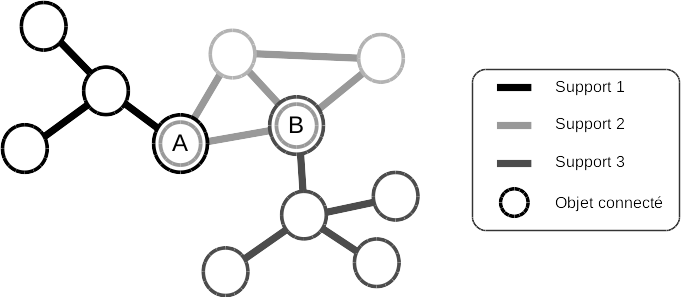
\includegraphics[width=.8\textwidth]{img/multinet.png}
         \caption{Exemple d'architecture réseau mélangeant plusieurs supports de communication.}
         \label{multinet}
      \end{figure}
      
      La figure \ref{multinet} est un exemple de réseau que notre protocole est capable de gérer. On
      peut voir qu'il permet de lier entre eux 3 supports de communication différents ayant 
		également des architectures de réseau différente. Le lien entre chacun de ces supports est
		réalisé par des objets connectés un peu particulier que l'on appelle des \emph{passerelles} 
		(\emph{A} et \emph{B} sur le schéma).
		Ces objets peuvent fonctionner de la même façon que n'importe quel autre objet. Ils ont
		cependant la possibilité de communiquer sur différents supports. Cela signifie que ces objets
		sont équipés au minimum de 2 technologies de communications. Par exemple, Wifi + Bluetooth,
		ZigBee + Ethernet ou même Wifi + Wifi (dans 2 réseaux différents).
		
	\subsection{Le routage}
% 		présentation du protocole VIP
% 		explication du transfert d’un message d’un support à un autre
% 		exemple concret d’un envoi de message
		Même avec une architecture de réseau comme celle de la figure \ref{multinet}, il faut laisser
		la possibilité à chaque objet de pouvoir communiquer avec n'importe quel autre objet. Cela ne
		sera pas aussi simple qu'avec une architecture ne contenant qu'un seul support.
		
		On va considérer que deux objets connectés sont \emph{voisins} s'ils appartiennent au même
		support de communication. On souhaite par exemple que l'objet \emph{C} envoi un message
		à l'objet \emph{F}. La première chose à faire est de déterminer qui est la cible. Étant donné
		que les deux objets appartiennent au même support, il suffit d'utiliser les adresses de 
		support de \emph{F} et\emph{C} (l'adresse MAC pour le Bluetooth, l'adresse IP pour le Wifi, 
		\dots). Le message sera alors
		transmit sans aucun problème puisque ce sera la technologie de communication qui s'occupera 
		du transport du message. Maintenant on souhaite que l'objet \emph{C} envoi un message à 
		l'objet \emph{G}. Cette fois-ci il va y avoir un problème puisque ces deux objets
		n'appartiennent pas au même support. L'utilisation des adresses de support ne servira à rien
		puisqu'elle ne seront pas compatibles. De plus, il est nécessaire de faire intervenir les
		objets \emph{A} et \emph{B} car ils font obligatoirement partie du transport du message.
		
		Ce problème a déjà été abordé lors de la création des premiers réseaux informatiques. Il 
		existe différentes solutions mais la plus connue est sans doute celle qui est actuellement 
		utilisée dans nos ordinateurs : le protocole IP. Cela signifie qu'il faut mettre en place un
		système similaire à celui qui relie les machines du monde entier. L'ensemble des objets
		connectés formera donc un \emph{réseau virtuelle} qui s'appliquera comme une surcouche aux
		technologies de communication existantes. Le nom de ce nouveau protocole des objets connectés
		est \emph{VIP} (Virtual Internet Protocol) imittant de façon simplifiée le protocole IP. Il
		est également accompagné du protocole VARP (virtual adress resolution protocol) qui sera 
		détaillé plus tard.
		
		\subsubsection{Le protocole VIP}
			Le protocole VIP définit pour chacun des objets une adresse VIP qui est composée de 3 
			octets (tableau \ref{vipFormat}). Chacun de ces octets possède une utilité précise. Le
			premier octet est utilisé pour référencer l'adresse du réseau. C'est une adresse globale
			qui sert à regrouper ensemble plusieurs sous-réseaux. En pratique, on utilise la même
			adresse de réseau pour la totalité des objets d'une maison. Cependant, si la maison
			possède plus de 64516 objets, il faudra au minimum 2 adresses de réseau pour représsenter
			une maison. Le deuxième octet de l'adresse VIP représente l'adresse de sous-réseau. C'est
			l'adresse d'un support de communication. Cela signifie que tous les objets d'un même
			support doivent utiliser la même adresse de sous-réseau. Encore une fois, s'il y a plus
			de 254 objets dans le même support, il faudra utiliser plusieurs adresses de support. Mais
			il faudra cependant ajouter des objets passerelles dans le même support pour que tous les
			objets puissent communiquer entre eux. Le dernier octet de l'adresse VIP va enfin définir
			l'adresse de l'objet. Cette adresse doit bien sûr être unique pour chaques objets d'un même
			sous-réseau.
			
			\begin{table}[ht]
				\centering
				\begin{tabular}{|l|l|l|}
					\hline
					Nom                         & Taille (bits) & Description              \\ 
					\hline\hline
					\texttt{ADDR{\_}NET}        & 8             & l'adresse de réseau      \\ \hline
					\texttt{ADDR{\_}SUB{\_}NET} & 8             & l'adresse de sous réseau \\ \hline
					\texttt{ADDR{\_}DEV}        & 8             & l'adresse de l'objet     \\ \hline
				\end{tabular}
				\caption{Format d'une adresse VIP}
				\label{vipFormat}
			\end{table}
			
			Il existe cependant des valeurs particulières d'adresse VIP : 
			\paragraph{Les adresses de réseaux}
				Toutes les addresses VIP dont l'adresse d'objet est 0 représente l'adresse du 
				sous-réseau. Cela signifie que l'adresse de décrit pas un objet mais le sous-réseau 
				lui-même. De la même façon, toutes les adresse VIP dont l'adresse de sous-réseau est 0 
				représente 	l'adresse de réseau (l'adresse doit valoir également 0).
				
			\paragraph{Les adresses de broadcast}
				Une adresse de broadcast est une adresse un peu particulière puisqu'elle représente la
				totalité des objets possédant le même réseau ou sous réseau que l'adresse de broadcast.
				Elle est définie avec la valeur maximale d'un ou plusieurs octets de son adresse VIP.
				Il faut cependant que ces octets soient les derniers de l'adresse.
				
			Les adresses VIP sont donc très similaire aux adresses IP. Elles n'ont cependant pas la
			même flexibilité puisque IP offre la possibilité de définir des masques de sous-réseaux
			dynamiques. Il y a également une différence au niveau de la représentation textuelle d'une
			adresse. Une adresse VIP s'écrit de la façon suivante : \\
			\makebox[\textwidth]{\texttt{ADDR{\_}NET:ADDR{\_}SUB{\_}NET:ADDR{\_}DEV}}
			en remplaçant chaque \texttt{ADDR} par sa valeur en hexadécimal. 
			Le tableau \ref{vipExample} montre quelques exemples d'adresse VIP.

			\begin{table}[!ht]
				\centering
				\begin{tabular}{ll}
					\texttt{0f:34:02} & objet 0x02 du sous-réseau 0x34 du réseau 0x02 \\
					\texttt{aa:b2:27} & objet 0x27 du sous-réseau 0xb2 du réseau 0xaa \\
					\texttt{aa:32:1c} & objet 0x1c du sous-réseau 0x32 du réseau 0xaa \\
					\texttt{23:00:00}	& adresse du réseau 0x23	\\
					\texttt{23:4b:00}	& adresse du sous-réseau 0x4b du réseau 0x23 \\
					\texttt{23:4b:ff}	& adresse de broadcast du sous-réseau précédent \\
					\texttt{23:ff:ff}	& broadcast à tous les objets du réseau 0x23 \\
					\texttt{ff:ff:ff}	& broadcast à tous le monde (à utiliser de faon modérée) \\
					\texttt{00:00:00}	& adresse du réseau virtuel (utile pour le routage) \\
				\end{tabular}
				\caption{Exemples d'adresses VIP.}
				\label{vipExample}
			\end{table}

			Avec ce système d'adresse pour les objets connectés, il est maintenant possible
			d'identifier de façon uniforme chaque objet du réseau virtuel mais également de pouvoir
			gérer la communication entre des objets de supports différents grâce au mécanisme de
			\emph{routage}. En effet, chaque objet est équipé d'une table que l'on appelle
			\emph{table de routage}. Ces tables permettent de définir le chemin que va	prendre un
			message entre un objet \emph{A} et un objet \emph{B}. Elles contiennent une liste 
			décrivant, pour chaque interface de communication d'un objet, l'adresse vers qui envoyer 
			les données en fonction du destinataire du message. Cela signifie que si l'on souhaite
			envoyer un message à une certaine adresse, le programme parcourra la table de routage à la
			recherche de la première règle qui correspondra à l'adresse. Le message sera alors envoyé
			à la passerelle associée la règle correspondante dans la table. Si aucune règle n'est
			adapté, il prendra la règle par défaut (adresse \texttt{00:00:00}). On peut également
			mettre des règles dont l'adresse de passerelle est \texttt{00:00:00}. Cela signifie que
			la passerelle est l'objet lui-même (c'est un réseau local à l'objet).
			
			Pour mieux comprendre ce mécanisme, prenons un exemple dans la figure \ref{vipNet}. L'objet
			\emph{C} souhaite envoyer un message à l'objet \emph{F}. Le tableau \ref{routingTable}
			donne la table de routage de chacun des objets connectés décrits dans la figure. La table
			qui nous intéresse dans cet exemple est celle de l'objet \emph{C} car il faut déterminer
			l'interface de communication qu'il faut utiliser pour émettre le message. Dans le cas de
			cet objet, la solution est vite trouvée puisqu'il ne possède qu'une seule interface :
			le support 1. L'adresse de l'objet \emph{F} est \texttt{01:4b:17}. L'objet \emph{C} va donc
			chercher l'adresse de réseau correspondante. La première ligne de la table concerne le
			réseau d'adresse \texttt{01:4b:00}. Cette ligne est déjà valide pour l'adresse de l'objet
			\emph{F}. Le message doit donc être envoyé à l'adresse de la passerelle de cette ligne.
			Il se trouve que l'adresse de passerelle est l'adresse par défaut. Cela signifie que l'on
			peut envoyer le message directement à l'objet \emph{F}. Il n'y a pas besoin de passer par 
			des intermédiaires.
			
			Maintenant, on va analyser l'envoi d'une message vers une destination plus lointaine.
			Prenons le cas de l'envoi d'un message entre l'objet \emph{C} et l'objet \emph{G}. 
			L'adresse de l'objet \emph{G} est \texttt{01:cc:42}. Dans la table de routage de \emph{C},
			la ligne concerné va être la deuxième puisque le réseau \texttt{01:cc:00} n'est pas connu.
			Il va donc envoyer le message à l'objet \emph{A} (la passerelle). Après réception du
			message par l'objet \emph{A}, celui-ci va lire sa table de routage pour chercher l'adresse
			de \emph{G}. La règle valide pour cette adresse est encore une fois la règle par défaut. Le
			message va donc être envoyer à l'objet d'adresse \texttt{01:e5:33} (l'objet \emph{B}).
			C'est ensuite au tour de \emph{B} de lire sa table de routage. Cette fois-ci le réseau
			\texttt{01:cc:00} est connue. La règle valide dans sa table est donc la deuxième. Le
			message sera ensuite envoyé à l'objet \emph{G}.
			
			\begin{figure}[!ht]
				\centering
				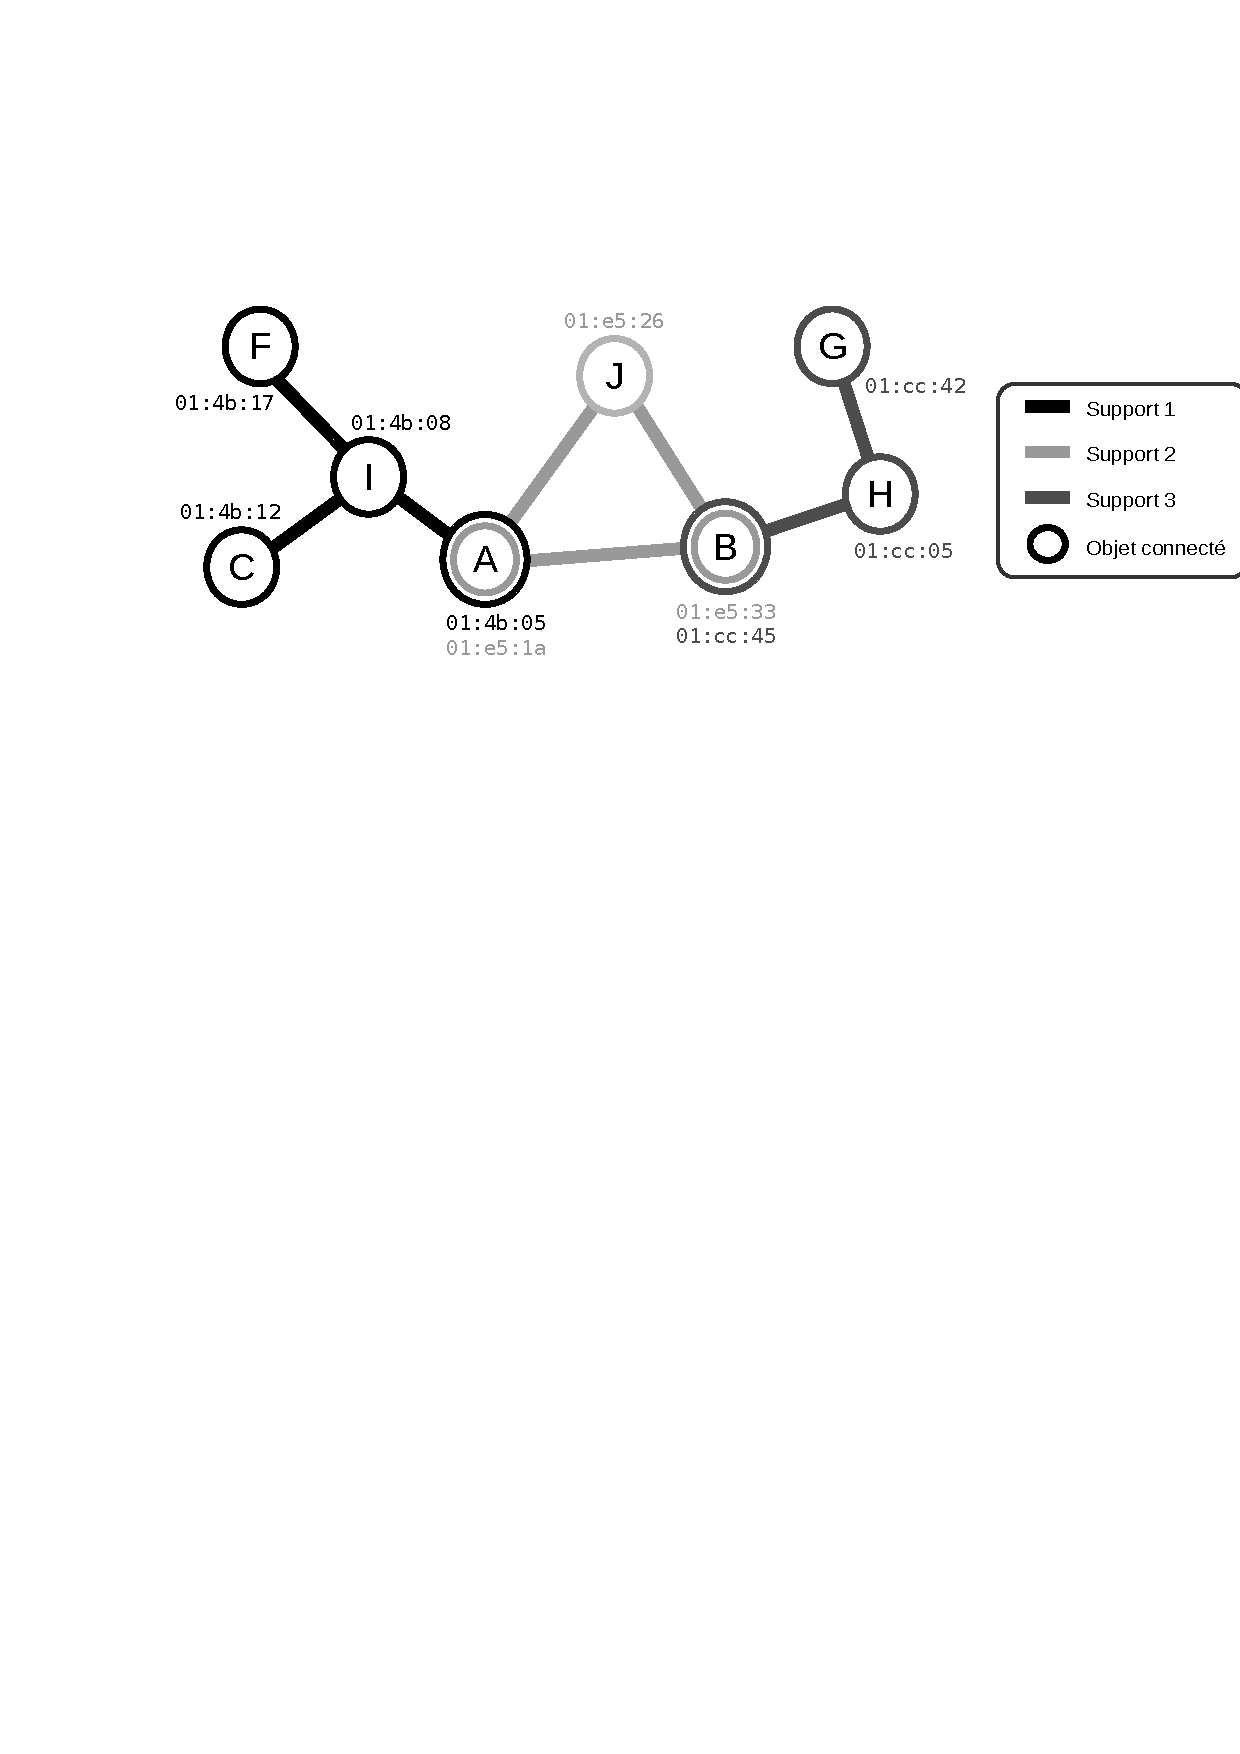
\includegraphics[width=\textwidth]{img/vip_net.png}
				\caption{Exemple de réseau en spécifiant les adresses VIP.}
				\label{vipNet}
			\end{figure}
			
			\begin{table}[!ht]
				\centering
				\begin{tabular}{|c|c|c|c|}
					\hline
					Objet              & Adresse de réseau & Passerelle        & interface \\ 
					\hline\hline
					\multirow{3}{*}{A} & \texttt{01:4b:00} & \texttt{00:00:00} & support 1 \\
					                   & \texttt{01:e5:00} & \texttt{00:00:00} & support 2 \\
					                   & \texttt{00:00:00} & \texttt{01:e5:33} & support 2 \\ \hline
					\multirow{3}{*}{B} & \texttt{01:e5:00} & \texttt{00:00:00} & support 2 \\
					                   & \texttt{01:cc:00} & \texttt{00:00:00} & support 3 \\
					                   & \texttt{00:00:00} & \texttt{01:e5:1a} & support 2 \\ \hline
					\multirow{2}{*}{C} & \texttt{01:4b:00} & \texttt{00:00:00} & support 1 \\
					                   & \texttt{00:00:00} & \texttt{01:4b:05} & support 1 \\ \hline
					\multirow{2}{*}{F} & \texttt{01:4b:00} & \texttt{00:00:00} & support 1 \\
					                   & \texttt{00:00:00} & \texttt{01:4b:05} & support 1 \\ \hline
					\multirow{2}{*}{G} & \texttt{01:e5:00} & \texttt{00:00:00} & support 3 \\
					                   & \texttt{00:00:00} & \texttt{01:cc:45} & support 3 \\ \hline
					\multirow{2}{*}{H} & \texttt{01:cc:00} & \texttt{00:00:00} & support 3 \\
					                   & \texttt{00:00:00} & \texttt{01:cc:45} & support 3 \\ \hline
					\multirow{2}{*}{I} & \texttt{01:4b:00} & \texttt{00:00:00} & support 1 \\
					                   & \texttt{00:00:00} & \texttt{01:e5:1a} & support 1 \\ \hline
					\multirow{2}{*}{J} & \texttt{01:e5:00} & \texttt{00:00:00} & support 2 \\
					                   & \texttt{00:00:00} & \texttt{01:e5:1a} & support 2 \\ \hline
				\end{tabular}
				\caption{Les tables de routage des différents objets de la figure \ref{vipNet}}
				\label{routingTable}
			\end{table}

			Comme l'on montré ces exemples, l'utilisation des tables de routage est un bon moyen pour
			transporter un message dans la totalité du réseau virtuel. Mais actuellement, elle possède
			un petit inconvénient. Il est nécessaire d'écrire les tables de routage de chacun des
			objets faisant passerelle. Il existe cependant des algorithmes de mise à jour dynamique
			des tables de routage mais ils n'ont pas encore été étudiés dans ce projet.

	\subsection{Un réseau dynamique}
		Le protocole VIP est suffisant pour mettre en place une architecture d'objets connectés dans
		une maison mais il manque cependant une étape pour que les messages puissent utiliser
		correctement les supports de communication. Imaginons que l'on souhaite envoyer un message 
		à un objet appartenant au même support. On connait on connait son adresse VIP. Mais comment 
		fait on pour déterminer à qui appartient l'adresse ? Il est en effet nécessaire de pouvoir 
		faire le lien entre l'adresse de support d'un objet et son adresse VIP. Pour cela, il a été
		mis en place un protocole nommé VARP (Virtual Address Resolution Protocol) inspiré du
		protocole ARP. Ce protocole permet d'effectuer des demandes d'adresses VIP ou d'adresses de
		support. Par exemple, si un objet est en possession d'une adresse de support, il peut
		récupérer l'adresse VIP correspondante avec une requête VARP. Et à l'inverse, il peut
		récupérer une adresse de support à partir d'une adresse VIP. Il est également possible de
		faire une requête multiple en utilisant une adresse de broadcast. Cela signifie que tous les
		objets acceptant cette adresse répondront à la requête. Cela peut par exemple être utilisé
		pour mettre à jour une table contenant la liste des couples d'adresses support/VIP des objets
		voisins. Le tableau \ref{varpEx} présente quelques exemples d'utilisation du protocole VARP.
		
		\begin{figure}[!ht]
			\centering
			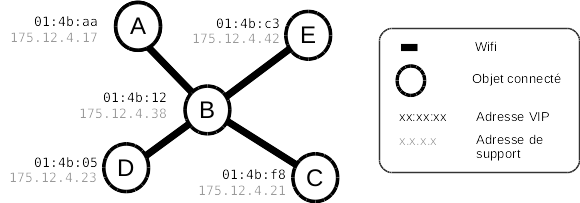
\includegraphics[width=\textwidth]{img/varp_net.png}
			\caption{Exemple de réseau Wifi d'objets connectés avec leurs adresses IP et VIP.}
			\label{varpNet}
		\end{figure}
		
		\begin{table}[!ht]
			\centering
			\begin{tabular}{|l|l|l||l|l|l|}
				\hline
				\multicolumn{3}{|c||}{Requête}     & \multicolumn{3}{|c|}{Réponse}  \\ \hline
				Objet & Demande & Adresse connue  & Objet & Adresse VIP & Adresse IP  \\ 
\hline\hline
				A     & IP      & 01:4b:f8        & C     & 01:4b:f8    & 175.12.4.21 \\ \hline
				A     & IP      & 01:4b:ff        & B     & 01:4b:12    & 175.12.4.38 \\
				      &         &                 & C     & 01:4b:f8    & 175.12.4.21 \\
				      &         &                 & D     & 01:4b:05    & 175.12.4.23 \\
				      &         &                 & E     & 01:4b:c3    & 175.12.4.42 \\ \hline
				A     & VIP     & 175.12.4.38     & B     & 01:4b:12    & 175.12.4.38 \\ \hline
				A     & VIP     & 255.255.255.255 & B     & 01:4b:12    & 175.12.4.38 \\
				      &         &                 & C     & 01:4b:f8    & 175.12.4.21 \\
				      &         &                 & D     & 01:4b:05    & 175.12.4.23 \\
				      &         &                 & E     & 01:4b:c3    & 175.12.4.42 \\ \hline
			\end{tabular}
			\caption{Exemple d'utilisation du protocole VARP par rapport à la figure \ref{varpNet}}
			\label{varpEx}
		\end{table}
		
		En faisant des scans réguliers en utilisant le protocole VARP, il est possible de détecter
		la connexion ou la déconnexion d'objets dans le réseau virtuel. Cela peut être pratique 
		pour rendre le réseau dynamique. Mais lorsqu'un nouvel objet se connecte au réseau, il faut
		cependant qu'il possède déjà une adresse VIP. De plus, cette adresse doit également respecter
		l'adresse de sous-réseau du support dans lequel il va se connecter. Sinon, il ne sera pas 
		possible de communiquer avec ce nouvel objet. La solution à ce problème serait d'affecter
		automatiquement une adresse VIP à chaque nouvel objet qui rejoint le réseau. Le protocole
		DHCP (Dynamic Host Configuration Protocol) à été conçu pour ça dans les réseaux Ethernet. Il
		faut donc créer un protocole similaire pour les objets connectés dans le réseau virtuel.
		Ce protocole n'a pas encore été étudié et n'est donc pas présent dans l'implémentation 
		actuelle du réseau virtuel.
		
		Avec la mise en place d'un système de connexion dynamique d'objets connectés, il est possible
		de mettre en place un nouveau type d'objet que l'on appelera \emph{objet mobile}. Ce genre
		d'objet doit pouvoir se déconnecter d'un sous-réseau lorsqu'il sort de sa portée mais il doit 
		également se connecter automatiquement aux réseaux qui sont dans sa proximité. Ils possèdent
		donc une adresse VIP variable. En utilisant un identifiant unique pour ces objets, il est
		possible de les localiser "grossièrement" dans la maison si l'on sait où sont placer les
		objets fixes. Cette information peut alors être utilisée pour effectuer des actions
		particulières dans des protocoles de plus haut niveau. Si l'on transforme des montres 
		intelligentes ou encore des smartphones en objet connecté, on peut alors déterminer la
		localisation d'une personne dans le réseau virtuel.
	
% 		apparition, disparition ou déplacement d’objets dans le réseau
% 		présentation du protocole VARP
% 		exemple d’apparition d’un objet
% 		les objets mobiles
%     aborder le protocole "pseudo DHCP" et expliquer qu'il n'est pas encore pensé
 
\section{La généricité des objets connectés}
	Avec les protocoles VIP et VARP, nous avons vu comment sont transportés les messages entre 
	n'importe quels objets du réseau virtuel. Il est temps maintenant de passer à un niveau plus haut
	et de s'intéresser à la composition de ces messages. 
	
	\subsection{Description d'un objet dans le protocole}
		Jusqu'à présent, tous les éléments du réseau virutel ont été décrit comme étant des objets
		connectés. On peut alors se demander pourquoi les différents noeuds du réseau sont qualifiés
		ainsi ? Quels sont leurs caractéristiques ? La définition d'un objet connecté a déjà été 
		abordé brièvement dans la première partie de ce rapport. Maintenant nous allons voir un peu
		plus en détails les fonctionnalités de ceux-ci. Tous ces éléments sont définis dans 
		un protocole encapsulé dans le protocole VIP : le protocole SDCP (Smarts Devices 
		Communication Protocol). Le tableau \ref{modeleCouche} illustre l'organisation des différentes
		couches du protocole de SmartDevCom.
		
		\begin{table}[!ht]
			\centering
			\begin{tabular}{r|c|c|c|}
				\cline{2-4}
				& & & Ethernet \\ \cline{4-4}
				Couche réseau & Bluetooth & ZigBee & IP \\ \cline{4-4}
				& & & UDP \\ \cline{2-4}
				\multirow{2}{*}{Couche réseau virtuel} & \multirow{2}{*}{VARP} & 
				\multicolumn{2}{c|}{VIP} \\ \cline{3-4}
				&                      & \multicolumn{2}{c|}{SDCP} \\
				\cline{2-4}
			\end{tabular}
			\caption{Représentation des différentes couches réseaux du protocole utilisé par 
					   SmartDevCom}
			\label{modeleCouche}
		\end{table}
		
		Le protocole permet de définir des objets connectés dont on ne connait pas la composition à 
		l'avance. Il est donc nécessaire de définir des règles permettant de décrire n'importe quel
		objet. Ce protocole doit alors essayer de rester le plus générique possible tout en offrant
		des fonctionnalités simples d'utilisation. Le protocole définit un objet connecté de la 
		manière suivante :
		\begin{itemize}
			\item il possède zéro, un ou plusieurs capteurs
			\item il possède zéro, un ou plusieurs actionneurs
			\item il possède zéro, une ou plusieurs actions
			\item il définit la façon dont doivent être utilisé chacune des actions
			\item il permet l'exécution de chacune de ses actions
		\end{itemize}
		
		Pour rappel, on considère ici qu'un capteur est un module d'un objet capable de mesurer une
		grandeur physique de son environnement. Un actionneur est un module capable d'agir sur son
		environnement. Une action représente une requête ou un ordre que l'on peut donner à un ou
		plusieurs des modules d'un objet. Étant donné que l'on ne connait pas forcément à l'avance
		à quoi correspond une action, il est nécessaire de définir précisément les paramètres qu'elle
		prend ainsi que les informations qu'elle retourne. L'ensemble des ces caractéristiques est
		récupérable à distance grâce à des requêtes définies dans le protocole SDCP. C'est justement
		cet ensemble de requêtes qui permet de pouvoir communiquer avec un objet sans avoir à
		connaitre au préalable à quoi il sert.
		
	\subsection{Méthode de classification des actions sur les objets}
% 		recherche des informations caractérisant les actions
% 		algorithmes de classification
		Pour pouvoir utiliser convenablement un objet inconnu, il est cependant nécessaire de pouvoir
		le ranger dans une certaine catégorie d'objet. En effet, on exécutera une de ses actions 
		uniquement si l'on sais à quoi elle sert. C'est pourquoir le protocole SDCP définit des types
		de capteurs, des types d'actionneurs et surtout des types d'actions. Dans cette architecture,
		connaitre le type des capteurs et des actionneurs d'un objet n'est pas quelque chose 
		d'indispensable. Lors de l'utilisation d'un objet, ce qui nous importe c'est l'exécution 
		des actions. Si l'on prend l'exemple d'un objet capable d'allumer la lumière en appuyant 
		sur un interrupteur mural. La demande de liste des actionneurs va retourner le servomoteur
		qui s'occupe de changer l'état du bouton. La demande de liste d'actions va retourner l'action
		permettant d'allumer ou d'éteindre la lumière. On remarque que le type de l'actionneur n'a
		que peu d'intérêt par rapport au type de l'action car ce dernier apporte une information bien
		plus précise.
		
		Mais le problème le plus important dans ce protocole est la définition des types des actions.
		Ce type doit valider deux contraintes : il doit définir précisément le rôle de l'action et
		il doit également être générique. Cela signifie par exemple que si un nouvel objet
		apparait dans le réseau avec un type d'action inconnu, les autres objets doivent pouvoir 
		comprendre de la façon la plus précise possible à quoi sert cette action. Cela pose demande
		donc beaucoup de réflexion sur la méthode à utiliser pour construire les types d'actions.
		
		Une solution intéressante pour résoudre ce problème serait de construire un arbre de type
		d'action. Cela permettrait de pouvoir définir des actions de façon très précise (lorsque l'on
		s'approche des feuilles de l'arbre) et également conserver un certain ordre d'idée pour 
		des types qui n'existe pas encore dans l'arbre (on connaitrait au moins l'une des branches de
		l'arbre). Mais la construction de cet arbre de type n'est, encore une fois, pas évidente.
		Pour cette construction, une première approche a été faite en utilisant des outils de
		statistique. Il existe en effet beaucoup d'algorithmes de clusterisation qui crée des
		structures sous forme d'arbre. Le problème de ces algorithmes est qu'ils utilisent des données
		quantitatives. Dans notre cas, les données sont pûrement qualitatives. Pour ce genre de
		données, une des méthodes consiste à lister un ensemble d'actions le plus varié possible et
		de rechercher des critères pouvant discriminer ces actions. Cette méthode est intéressant mais
		la recherche des critères discriminant est presque aussi compliqué que d'essayer de construire
		l'arbre des types à la main.
		
		Finalement, l'arbre des types d'actions a été écrite manuellement en essayant de faire le tour
		des types d'actions que l'on peut potentiellement rencontrer avec des objets connectés. Voici
		un extrait de la liste des types d'actions actuellement gérées (le vrai arbre est sur 4 
		niveaux) :
		\begin{itemize}
			\item ambiance
			\begin{itemize}
				\item action kinéstésique
				\item action visuelle
				\item action auditive
			\end{itemize}
			\item sécurité
			\item multimédia
			\begin{itemize}
				\item audio
				\item vidéo
			\end{itemize}
			\item électroménager
			\begin{itemize}
				\item alimentaire
			\end{itemize}
			\item accessibilité (humain)
			\begin{itemize}
				\item déplacement
				\item ouverture de porte
				\item localisation
			\end{itemize}
			\item entretien
		\end{itemize}

	\subsection{Gestion dynamique d’objets}
% 		comment un objet d’un nouveau type peut s’intégrer à la hiérarchie
% 		les différentes solutions d’intégration
% 		exemple
		Cette méthode de gestion des types d'actions est déjà suffisante pour la plupart des objets
		que l'on serait susceptible de créer. Mais il est cependant possible d'aller encore plus loin
		en créant des objets spéciaux agissant comme des bases de données. Ces objets auront pour
		tâche de mettre à jour un arbre de type regroupant tous les types que l'on peut rencontrer
		dans le réseau virtuel. Cette base sera bien évidemment dynamique pour que des nouveaux objets
		puissent ajouter de nouveau type. Ces objets peuvent également rassembler d'autres types de
		données comme par exemple la liste des actions de tous les objets. Ce regroupement
		d'informations peut être très utile pour d'autres objets dont l'unique but est de contrôler
		des objets existants.
		
		Le protocole SmartDevCom réunit assez d'outils pour pouvoir créer des objets connectés très 
		variés. Il permet d'avoir une structure solide sur laquelle on peut alors mettre en place 
		tout une hiérarchie d'objets connectés allant du simple objet appuyant sur un bouton jusqu'à
		des objets intégrant de l'intelligence artificielle et dédié au contrôle des autres objets.
		Il n'y a alors plus aucune limite dans la dynamicité et la réactivité du réseau virtuelle.


   \clearemptydoublepage
   
   \chapter{La création des objets}

\section{Reconnaissance vocale : Application Android}
	\subsection{Etat de l’art}	
Tout projet implique une phase de recherche, afin d'effectuer un état de l'art sur ce qu'il a déjà été fait auparavant dans ce domaine. Afin de rechercher ce qu'il fallait pour cet état de l'art, il a donc fallu décomposer en plusieurs parties ce que devait réellement réaliser cette reconnaissance. Ces parties étaient :

\begin{itemize}
\item Activation de la reconnaissance vocale automatiquement
\item Gestion de la chaîne de caractères comprise par la reconnaissance
\end{itemize}

De base sur Android, il est possible d'activer la reconnaissance vocale  automatiquement grâce aux mots clefs 
« OK Google ». Souhaitant appeler notre intelligence domotique Jarvis, il était peu souhaitable de dire ces mots afin d'activer la reconnaissance.
Après recherches, il s'avère qu'il n'existe aucun moyen simple de changer ces mots clefs, puisque les seuls moyens sont soit d'avoir un téléphone rooté, autrement dit où l'on a tous les accès afin de changer le bon fichier de configuration. Soit d'avoir un téléphone de la marque Motorola, qui intègre le changement de ces mots directement dans son firmware. C'est pourquoi pour activer la reconnaissance vocale, nous sommes obligés de prononcer les mots « OK Google ».
	
	\subsection{Activation de la reconnaissance vocale}
	
Afin de pouvoir démarrer et utiliser la reconnaissance vocale, il faut un ensemble d'éléments :
\begin{itemize}
 \item Autovoice
 \item Tasker
\end{itemize}

\begin{figure}[!ht]
         \centering
         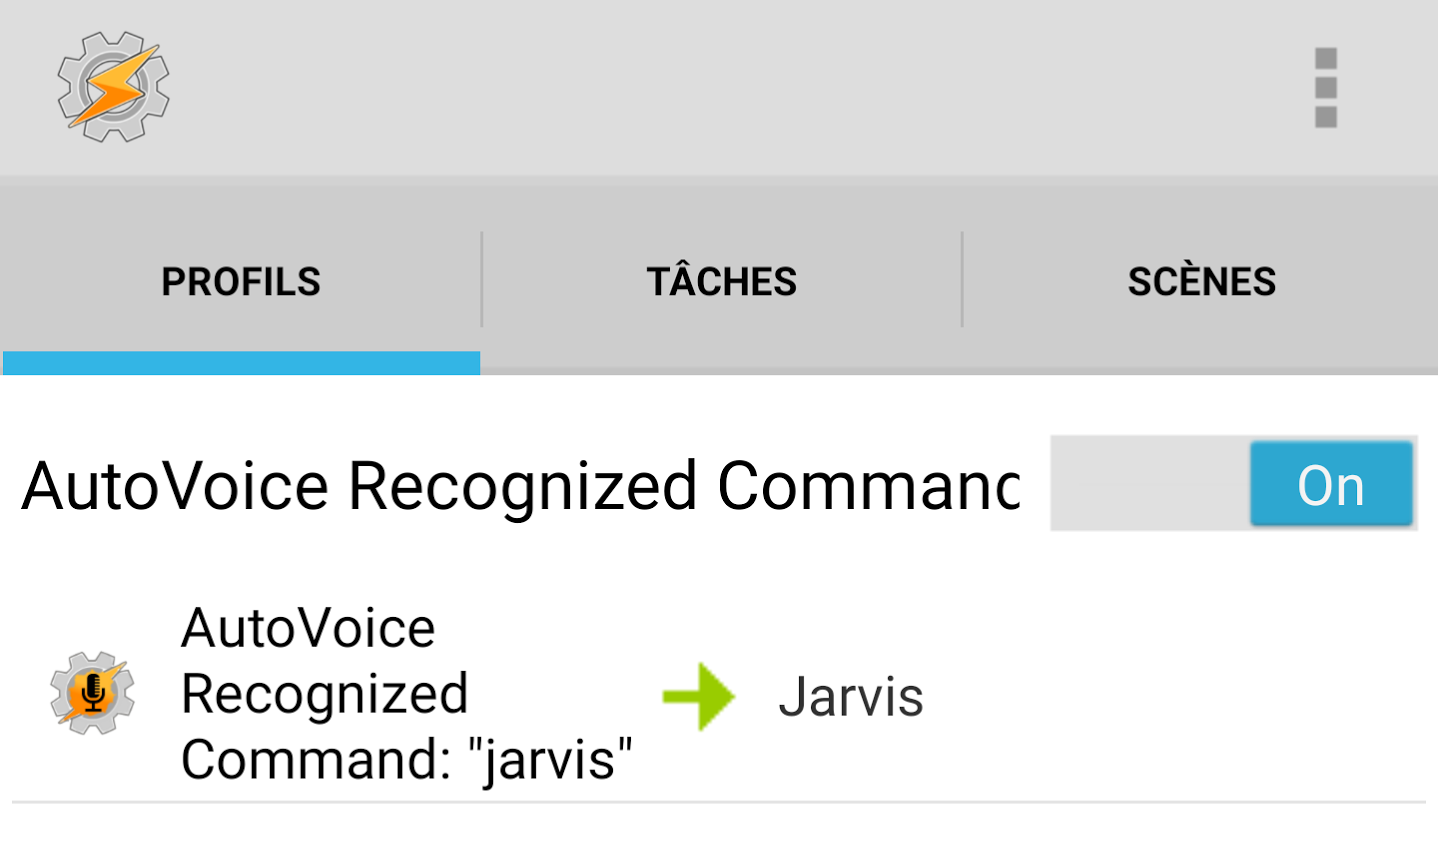
\includegraphics[width=0.5\textwidth]{img/tasker.png}
         \caption{Autovoice + Tasker}
         \label{Tasker}
\end{figure}

Autovoice est une application Android qui permet d'utiliser la reconnaissance vocale de Google, et 
de se servir de la chaîne de caractères reconnues pour en faire ce que l'on souhaite. Par ailleurs, 
on peut la paramétrer de telle sorte qu'elle réagisse seulement si une suite de mots clefs est 
reconnue, comme sur la figure \ref{Tasker}. Afin de pouvoir communiquer avec Jarvis, le seul mot 
clef choisi a donc été son nom. Du côté de Tasker, c'est une application d'automatisation très 
connue sur Android. Elle permet de réaliser des tâches en réponse à un événement donné. Ainsi il est 
possible d'utiliser comme événement Autovoice, et comme tâche, une application qui permet de traiter 
la chaîne de caractères : SpeechToText, comme on peut le voir 
sur la figure \ref{jarvis}.

\begin{figure}[!ht]
         \centering
         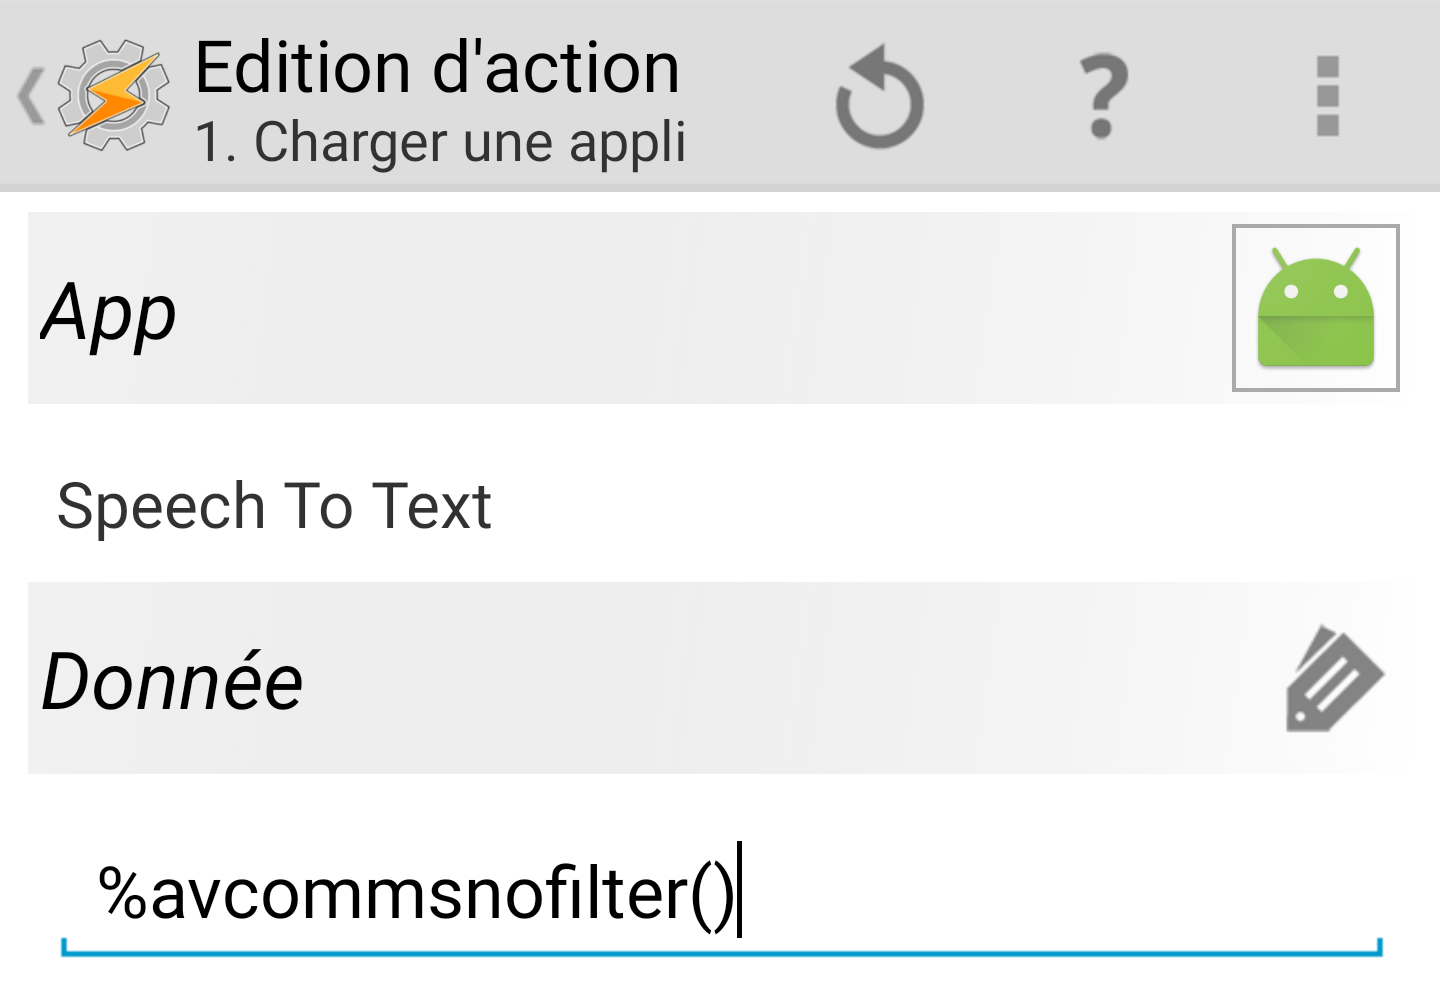
\includegraphics[width=0.5\textwidth]{img/jarvis.png}
         \caption{Tâche jarvis}
         \label{jarvis}
\end{figure}

	\subsection{SpeechToText}
	
	  \subsubsection{La base de données}
	
SpeechToText est une application Android qui permet donc d'interpréter une chaîne de caractères, et d'envoyer une trame suivant le protocole SDCP au bon objet connecté. L'application possède deux bases de données dynamiques. La première possède l'ensemble des objets intelligents. Cette base de données est stockée dans un fichier JSON.

\begin{figure}[!ht]
         \centering
         	\begin{lstlisting}
{
    "smartDevices" : [
      {
	"device": {
	  "idAction": "0x111",
	  "bleName": "sdc_Lisa"
	}
      }]
}
		\end{lstlisting}
         \caption{Base de données des objets intelligents}
         \label{BDD_smart}
\end{figure}


Cette base de données comprend une liste des objets connectés proches de nous. Comme on peut le voir un objet est caractérisé par deux choses : l'identifiant de l'action qu'il peut réaliser, ainsi que le nom de l'objet bluetooth auquel il faut se connecter pour réaliser l'action.

\begin{figure}[!ht]
         \centering
	 \begin{lstlisting}[caption=][frame=single]
{
    "voiceCommands" : [
      {
        "command" : {
            "voiceActivation" : "Quelle est la temperature",
            "voiceDiction" : "la temperature est",
            "idAction" : "0x111"
        }
      }]
}
	 \end{lstlisting}
         \caption{Base de données des commandes vocales}
         \label{BDD_objects}
\end{figure}



Ainsi une commande vocale est caractérisée par une chaîne de caractères à reconnaître, une chaîne de caractères à dire par synthèse vocale, afin de donner un feedback sur ce qu'il se passe à l'utilisateur. Elle contient elle aussi l'identifiant de l'action à réaliser, afin de faire le lien avec l'autre base de données.

Dès que la phrase est analysée par la reconnaissance vocale, il est nécessaire de reconnaître la requête que l'utilisateur souhaite réaliser. Pour ce faire, l'application réalise un algorithme sur la chaîne reçue, dont le but est d'évaluer la similarité avec l'ensemble des phrases possibles. La distance minimale caractérisera la requête faite par l'utilisateur. Il existe différents algorithmes, tel que: Levenshtein, ou JaroWinkler.

    \subsubsection{La distance de Levenshtein}
C'est le plus simple des deux algorithmes. Cette distance calcule le nombre de différences qu'il y a entre deux chaînes de caractères. Ces différences peuvent être le remplacement, la suppression, ou l'insertion d'un caractère.

    \subsubsection{La distance de JaroWinkler} 
Celle-ci part de la distance de Jaro dont l'équation est [1]: 
\begin{equation}
 d = \frac{1}{3}(\frac{m}{|s1|}+\frac{m}{|s2|}+\frac{m-t}{m})
\end{equation}

où :
\begin{itemize}
 \item $|s_i|$ est la longueur de la chaîne de caractères de la chaîne 'i'
 \item $m$ est le nombre de caractères \emph{correspondants} dans les 2 chaînes
 \item $t$ est le nombre de \emph{transpositions} nécessaires de ces caractères partagés
\end{itemize}

Deux caractères identiques de $s_1$ et $s_2$ sont dit \emph{correspondants} lorsque leur éloignement dans 
leur chaîne respective ne dépasse pas :
\begin{equation}
 \lfloor{\frac{max(|s_1|, |s_2|)}{2}}\rfloor - 1
\end{equation}

Le nombre de \emph{transpositions} est obtenu en comparant le i-ème caractère \emph{correspondant} de $s_1$ avec le i-ème caractère \emph{correspondant} de $s_2$. Le nombre de fois où ces caractères sont différents, divisé par deux, donne le nombre de transpositions.

On calcule ensuite la distance avec cette équation :
\begin{equation}
 d_w = d_j + (l_p(1-d_j))
\end{equation}

avec :
\begin{itemize}
 \item $d_j$, la distance de Jaro entre $s_1$ et $s_2$
 \item $l$, la longueur du préfixe commun (avec un maximum de 4 caractères)
 \item $p$, un coefficient qui permet de favoriser les chaînes avec un préfixe commun. Winkler propose 
pour valeur $p=0.1$.

\end{itemize}

Wikipédia donne un très bon exemple pour comprendre cette distance. Ils appliquent cette algorithme pour 
calculer la distance entre MARTHA et MAR\underline{HT}A. Pour cela ils dressent un tableau :

\begin{figure}[!ht]
         \centering
	    \begin{tabular}{|0|1|2|3|4|5|6|}
		\hline
		& M & A & R & T & H & A \\
		\hline
		M & 1 & 0 & 0 & 0 & 0 & 0 \\
		\hline
		A & 0 & 1 & 0 & 0 & 0 & 0 \\
		\hline
		R & 0 & 0 & 1 & 0 & 0 & 0 \\
		\hline
		H & 0 & 0 & 0 & 0 & \textbf{1} & 0 \\
		\hline
		T & 0 & 0 & 0 & \textbf{1} & 0 & 0 \\
		\hline
		A & 0 & 0 & 0 & 0 & 0 & 1 \\
		\hline
	      \end{tabular}
         \caption{Exemple pour la distance de JaroWinkler}
         \label{JaroWinkler}
\end{figure}

On a :
\begin{itemize}
  \item $m = 6$ (Nombre de 1 dans la matrice)
  \item $|s_1| = 6$ 
  \item $|s_2| = 6$
  \item Les caractères correspondants sont \{{M,A,R,T,H,A\} pour $s_{1}$ et \{{M,A,R,H,T,A\} pour $s_{2}$. 
\end{itemize}

On a donc 2 couples (T/H et H/T) de caractères \emph{correspondants} différents, soit deux 
demi-transpositions. D'où $t=\frac {2}{2}=1$.

La distance de Jaro est :

\begin{equation}
 d_j = \frac {1}{3}\left(\frac {6}{6}+ \frac {6}{6}+\frac {6-1}{6}\right)=0.944
\end{equation}

La distance de Jaro-Winkler avec $p=0.1$ avec un préfixe de longueur $\ell =3$ devient

\begin{equation}
  d_w=0.944+(3*0.1(1-0.944))=0.961
\end{equation}

\subsubsection{Etude de l'algorithme le plus approprié}
La meilleure distance pour notre projet a été trouvée en faisant une série de tests, en utilisant à chaque 
fois les deux algorithmes. Le test consiste à prendre plusieurs phrases présentes dans le fichier des 
commandes vocales, et à les dire un grand nombres de fois, avec différents tons de voix, 
différentes 
articulations, et différents volumes. Ensuite, pour chacune de ces requêtes, une liste des différentes 
phrases comprises par la reconnaissance vocale est établie. Les deux algorithmes sont alors appliqués, pour 
voir lequel est le plus robuste, et nous donne la correspondance la plus grande entre la requête souhaitée, et 
les commandes comprises. Il s'avère que l'algorithme le plus simple  était le plus robuste pour notre étude, 
c'est donc la distance de Levenshtein qui a été gardée. 

Maintenant que nous sommes capables de savoir quelle requête l'utilisateur souhaite envoyer, et à quel objet, 
il faut savoir comment l'envoyer.

	\subsection{Intégration du protocole avec JNI}
Le protocole a été construit pour être sur systèmes embarqués, avec le langage C++. Or l'objet reconnaissance 
vocale doit lui aussi l'utiliser afin de pouvoir communiquer convenablement avec les autres objets. Ainsi deux 
choix étaient possibles :
\begin{itemize}
 \item Réécrire le protocole sous Android
 \item Intégrer le protocole en réalisant une interface pour Android
\end{itemize}

C'est la deuxième option qui a été choisie, celant évitant de refaire une grosse partie du travail déjà 
réalisée.

Il faut savoir que le système Android fonctionne grâce à une machine virtuelle Java : \emph{Art} (Pour 
Android Run Time). Cette machine n'exécute de base à priori que du byte code Java, et non de l'assembleur que 
l'on pourrait obtenir en compilant un langage natif comme le C++. Grâce à \emph{JNI}, pour Java Native 
Interface, il est possible d'interfacer du code java, avec du code natif. Pour cela il suffit de compiler le 
code natif pour en faire une bibliothèque, qu'il suffira se charger dans le programme. Cette 
bibliothèque
contient un ensemble de fonctionnalités déjà compilé, et qui peut donc être utilisé directement dans le 
programme.

\subsubsection{Intégration de la bibliothèque [2]}
La première chose à faire est de créer une classe dans le code Java, elle contiendra plusieurs directives 
importantes, comme le chargement de la bibliothèque, mais aussi le prototype de la fonction 
\emph{fromCpp} qui 
sera défini dans le code natif, cela permettra de créer le lien entre les deux langages. Il faut ensuite 
demander au compilateur java de créer un fichier d'en-tête à partir de cette classe, qui sera utilisée dans 
notre bibliothèque plus tard.

Il faut ensuite écrire le corps de la fonction \emph{fromCpp}, dans un autre fichier C++. Afin de faire le 
lien avec le code java, il faut inclure le fichier d'en-tête tout juste créé. Par la suite, nous devons 
compiler ce code en précisant que nous souhaitons obtenir une bibliothèque et pas un fichier 
exécutable. Cela 
nous donnera un fichier \emph{.so} sous Linux, ou un fichier \emph{.dll} sous Windows. Ce fichier devra 
être placé à la racine du projet, afin que la machine virtuelle java puisse le trouver pendant l'exécution.

Dès lors il sera possible d'utiliser du code natif, et donc de pouvoir se servir du protocole afin 
de pouvoir communiquer avec les différents objets, et cela grâce au bluetooth d'Android.


	\subsection{Communiquer avec le protocole BLE}
	  \subsubsection{Fonctionnement du BLE}
L'application Android a donc pour but d'utiliser le protocole Bluetooth Low Energy (BLE), pour 
transmettre les 
paquets aux différents objets connectés. Afin de pouvoir se servir de ce bluetooth, il faut commencer par 
effectuer un scan pour lister tous les objets supportant ce protocole aux alentours. Une fonction 
de callback est appelée pour chaque appareil détectée. On peut ensuite se connecter à cet appareil, 
afin d'être appairé avec celui-ci.

Tous les appareils utilisant le protocole BLE utilisent le GATT (\emph{Generic Attribute Profile}), afin 
d'envoyer et recevoir des données sur le réseau. Il faut donc obtenir cette interface pour pouvoir 
communiquer en BLE. Une fois l'interface GATT obtenue, il est possible de récupérer l'ensemble des 
caractéristiques. Les caractéristiques sont l'ensemble des valeurs de l'appareil que l'on peut lire 
ou écrire. Elles sont composées d'un UUID (\emph{Universally Unique Identifier}), d'une propriété qui permet 
d'avoir une description lisible de la caractéristique, et enfin d'une valeur. Par conséquent, si l'on souhaite 
obtenir la valeur de température d'un objet, il faut récupérer la caractéristique dont la propriété est 
"température", puis simplement récupérer sa valeur.

Cette procédure ne peut être simplifiée, il est donc obligatoire d'effectuer un scan pour voir l'ensemble des 
objets bluetooth dans les environs, même si nous les connaissons déjà. Il est donc impossible via le BLE 
d'android de se connecter directement à un appareil à partir de son adresse MAC bluetooth, ce qui est 
dommage, car nous devons obligatoirement réaliser un scan, afin de communiquer avec un objet 
proche de nous, même si nous le connaissons.


\section{Les objets intelligents}

Maintenant que les différentes briques ont été posées, il est possible de créer les différents objets
intelligents.

\begin{figure}[!tbp]
  \centering
  \begin{minipage}[b]{0.49\textwidth}
    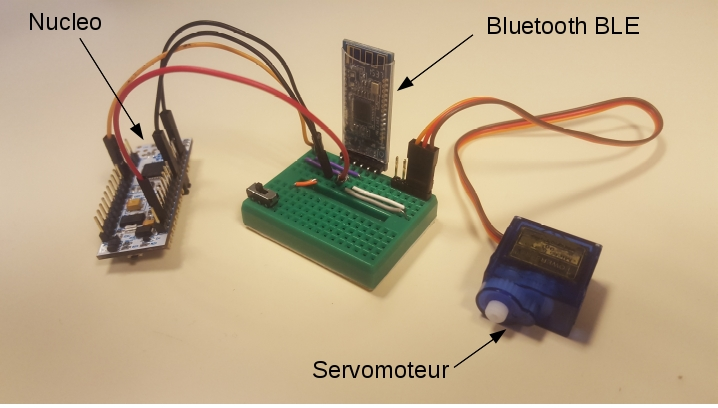
\includegraphics[width=0.95\textwidth]{img/actuator2.jpg}
    \caption{Actionneur intelligent}
    \label{actuator}
  \end{minipage}
  \hfill
  \begin{minipage}[b]{0.49\textwidth}
    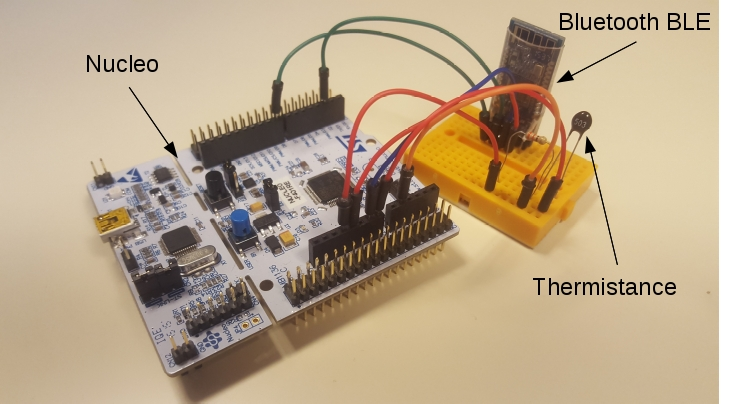
\includegraphics[width=0.95\textwidth]{img/sensor2.jpg}
    \caption{Capteur intelligent}
    \label{sensor}
  \end{minipage}
\end{figure}

Il est possible de voir sur les figures \ref{actuator} et \ref{sensor} que les deux objets ne possèdent pas la 
même carte de développement Nucleo. La carte présente pour l'actionneur est une F303K8, tandis que celle du 
capteur est une F401RE. De manière générale, la première possède moins de composants, mais est plus petite, 
ce qui est largement suffisant pour la création de nos objets connectés.

L'actionneur présent sur la figure \ref{actuator} est composé d'un servomoteur. Cet objet a été utilisé en 
tant qu'interrupteur intelligent. Le capteur présent sur la figure \ref{sensor} est quant à lui composé d'une 
thermistance, afin de pouvoir récupérer la température de la pièce.




   \clearemptydoublepage
   
   \chapter*{Conclusion}

Le but de ce projet était de mettre en place un réseau d'objets connectés équipés de capteurs et
d'actionneurs dédiés à la domotique. Mais pour pouvoir réaliser ce genre de réseau, il est 
indispensable de mettre en place un protocole de communication pour que tous les objets se
comprennent. Étant donné que souhaitions avoir aucune contrainte lors de la création des objets
connectés, il a fallu écrire un protocole qui soit le plus générique et dynamique possible. C'est
pourquoi la tâche la plus importante du projet a été la mise en place du protocole.
Actuellement, celui-ci est opérationnel bien qu'il n'intègre pas encore toute la dynamique que
nous souhaitions.

Ce projet a donc nécessité une grande partie de réflexion et d'analyse pour concevoir un protocole 
générique. Il a requis beaucoup de connaissances dans le domaine du réseau mais également un peu
dans le domaine des statistiques pour l'organisation des types d'actions. Mais le projet n'a pas été
uniquement théorique. L'implémentation du protocole et la création d'objets ont fait intervenir des
technologies assez récente comme la norme C++14 pour le protocole, la cross-compilation avec Docker 
pour programmer sur ARM, JNI pour intégrer du code natif sous Android, des outils de programmation
temps réel ainsi que des bibliothèques d'Android et d'Mbed. Ce projet a donc été très enrichissant 
d'une part, pour les nombreux domaines de l'informatique embarqué qu'il a fait intervenir et d'autre
part, pour la fusion et la concrétisation de beaucoup de connaissances que l'on a acquise à l'ISIMA.
Cet enrichissement ne va cependant pas s'arrêter là puisque l'étape suivante est maintenant la 
création de vrais objets qui utiliseront le travail qui a été réalisé dans ce projet.
				
   \clearemptydoublepage
   
   \chapter*{Perspectives}

Beaucoup de choses ont été faites dans ce projet, mais il reste encore plus de choses à faire avant
de pouvoir obtenir un vrai réseau d'objets pour la domotique.

\section*{Dynamicité du protocole}
	Avec l'ensemble des outils qui a été défini par les protocoles VIP, VARP, VDHCP et SDCP. Il 
	est théoriquement possible de créer tous les objets que l'on peut imaginer. Mais le protocole
	n'est pas encore complètement implémenté. Il manque encore la gestion dynamique des tables de
	routage, la création du protocole VDHCP (pour l'affectation automatique d'adresse VIP) et la 
	gestion des interfaces Wifi. Si l'on souhaite pouvoir profiter pleinement des fonctionnalités
	du protocole, il est donc indispensable de l'implémenter complètement pour bénéficier d'un
	réseau virtuel dynamique.

\section*{Création d'un réseau virtuel}
	La plus grande partie du projet a été consacrée à la réalisation du protocole. Mais la partie
	la plus intéressante est cependant lorsque l'on commence à créer un ensemble d'objets et de les
	mettre en réseau. On atteint alors une étape beaucoup plus visuelle et donc beaucoup agréable 
	pour travailler. Malheureusement il était indispensable de mettre d'abord en place les briques
	de base du protocole avant de pouvoir commencer un objet. Mais une fois ces problèmes
	réglés, il sera alors possible d'équiper entièrement un ensemble de maisons en domotique, afin de 
	créer ce réseau virtuel.

\section*{Ajout d'une intelligence}
	Une fois qu'a été mis en place un réseau virtuel contenant un ensemble suffisant d'objets 
	connectés, on a alors la possiblité d'obtenir des informations sur la maison ou d'effectuer
	certaines actions. Mais à ce niveau là, on peut alors monter d'un cran l'intelligence de la
	maison en créant des objets capables d'analyser les données des autres objets et de pouvoir
	effectuer des actions en conséquence. Cela signifie que l'on peut mettre en place une sorte
	d'intelligence artificielle dans certains objets. La maison serait alors capable d'anticiper
	certaines des requêtes des utilisateurs.

\section*{Création d'un logiciel intégré}
	Ce logiciel permettra d'automatiser la création de tous les objets connectés possibles. Il 
	contiendra une base de données de tous les objets que l'on peut créer, avec la liste de leurs 
	différents 	capteurs et actionneurs. Cette base de données contiendra la références de ces 
	modules afin de pouvoir les 	commander sur Internet sur des sites de références. Enfin, il 
	permettra d'envoyer le bon programme sur l'objet automatiquement.

				
   \clearemptydoublepage
   
   \frontmatter   % Numérotation romaine minuscule
   \chapter*{Lexique}
   \clearemptydoublepage
   
   \chapter*{Bibliographie}
   \clearemptydoublepage
   
   \renewcommand{\thesection}{\Alph{section}}
   \setcounter{section}{0}
   
   \let\origappendix\appendix % save the existing appendix command
   \renewcommand\appendix{\clearpage\pagenumbering{Roman}\origappendix}
   
   \appendix
   
%    \chapter{Diagramme de Gantt}
%       {\centering
%       \includegraphics[width=.8\textwidth]{}}

\end{document}

